Space Cobot \cite{roque2016space} is a holonomic, multirotor modular vehicle designed with modularity for easy maintenance and a wide range of applications. The propulsion system consists of six electric motors arranged to ensure holonomic kinematics.

Each motor in the propulsion module is 4.5 inches in size and operates independently. The configuration of these motors guarantees that the robot maintains holonomic dynamics. It is crucial to consider the bidirectional capability of the motors; although they can exert force in both directions, a slight reduction in thrust occurs when the associated propeller spins in reverse.

For a single propeller \(i\), which is rigidly linked to the robot's body frame (see Figure \ref{fig:Proposed Approach: Space Cobot: Motor graph}), both the thrust (\(F_{i}\)) and the torque (\(M_{i}\)) can be computed using the following equations. Here, \(u_i\) represents the input of the \(i\)-th actuator in rpm (rotations per second), \(K_1\) is the thrust coefficient, \(K_2\) is the torque coefficient, and \(w_i\) is either \(+1\) or \(-1\), depending on whether the propeller rotates clockwise (CW) or counterclockwise (CCW). Note that \(w_i \neq \omega\), where \(\omega\) denotes the robot's angular velocity.

\begin{figure}[H]
    \centering
    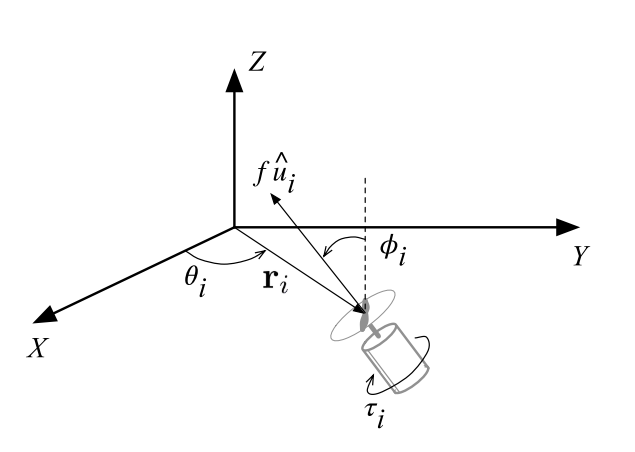
\includegraphics[width=0.7\textwidth]{Images/Propposed Aproach/space cobot motor graph.png}
    \caption{Notation used for modeling a single propeller in the Space Cobot robot. Image sourced from \cite{roque2016space}.}
    \label{fig:Proposed Approach: Space Cobot: Motor graph}
\end{figure}

\begin{align}
    F_{i} &= f_i, & f_i &= K_{1} u_i, \\
    M_{i} &= \bar{r}_{i} \times F_{i} - \tau_{i} u_i, & \tau_{i} &= w_i K_{2} u_i
    \label{eq:Proposed Approach: Space Cobot: Motor equations}
\end{align}

The constants \(K_1\) and \(K_2\) are defined as follows (Equation \ref{eq:Proposed Approach: Space Cobot: Motor constants}), where \(\rho\) is the air density, \(D\) is the propeller diameter, and \(C_T\) and \(C_P\) are the thrust and power coefficients, respectively (dimensionless) \cite{mccormick1994aerodynamics}.

\begin{align}
    K_{1} &= \rho D^{4} C_{T}, & K_{2} &= \frac{\rho D^{5} C_{P}}{2\pi}
    \label{eq:Proposed Approach: Space Cobot: Motor constants}
\end{align}

Referring again to Figure \ref{fig:Proposed Approach: Space Cobot: Motor graph}, the position and orientation of each propeller relative to the center of mass (COM) of the robot are given by Equation \ref{eq: Proposed Approach: Space Cobot: Motor position and orientation}:

\begin{align}
    \bar{r}_{i} &= \begin{bmatrix}
        d \cos(\theta_{i}) \\ 
        d \sin(\theta_{i}) \\
        0
    \end{bmatrix}, &
    \hat{u}_{i} &= \begin{bmatrix}
        \sin(\theta_{i}) \sin(\Phi_{i}) \\
        -\cos(\theta_{i}) \sin(\Phi_{i}) \\
        \cos(\Phi_{i})
    \end{bmatrix}
    \label{eq: Proposed Approach: Space Cobot: Motor position and orientation}
\end{align}

Using general robot dynamics, we can stack the forces and moments applied to the robot and relate them to the actuation of all motors. By this logic, we derive a linear relation where:
\[
\begin{pmatrix} F_{i} \\ M_{i}  \end{pmatrix} = \hat{a}_{i} u_{i}
\]
Here, \(\hat{a_i}\) represents the actuation vector of the \(i\)-th motor, which is defined in Equation \ref{eq:Proposed Approach: Space Cobot: Actuation vector}, it should be noted that the value of  \( \bar{r}_i \) is referenced to the center of mass of the robot, and not the geometrical center of the propellers. For the robot to maintain holonomic behavior, the configuration of the actuators must ensure that matrix \(A\) is at least rank 6. The selected configuration is shown in Table \ref{tab:Proposed Aproach: Space Cobot Motor and propeller configuration}.

\begin{equation}
\mathbf{a}_i = 
\begin{pmatrix}
K_1 \sin(\theta_i) \sin(\phi_i) \\
-K_1 \cos(\theta_i) \sin(\phi_i) \\
K_1 \cos(\phi_i) \\
[K_1 \bar{r}_i \cos(\phi_i) - w_i K_2 \sin(\theta_i)] \sin(\phi_i) \\
-[K_1 \bar{r}_1 \cos(\phi_i) - w_i K_2 \sin(\phi_i)] \cos(\theta_i) \\
-K_1 \bar{r}_i \sin(\phi_i) - w_i K_2 \cos(\phi_i)
\end{pmatrix}
\label{eq:Proposed Approach: Space Cobot: Actuation vector}
\end{equation}

\begin{table}[H]
\centering
\begin{tabular}{c|cccccc}
Propeller (\(i\)) & 0  & 1   & 2   & 3    & 4   & 5   \\ \hline
\(\theta_{i}\)     & 0  & 60  & 120 & 180  & 240 & 300 \\
\(\Phi_{i}\)       & 55 & -55 & 55  & -55  & 55  & -55 \\
\(w_{i}\)          & -1 & 1   & -1  & 1    & -1  & 1   \\ \hline
\end{tabular}
\caption{Configuration of Propeller Placement in Space Cobot. The values of \( \theta_{i} \) and \(\Phi_{i} \) are in degrees. The values of \(w_{i}\) are either -1 or 1, depending on the propeller's rotation direction.}
\label{tab:Proposed Aproach: Space Cobot Motor and propeller configuration}
\end{table}

To accurately model the relationship between the input signal \( u \) (rad/s, radians per second) and the resulting thrust and torque, real-world data from both the motor and the propeller were required. To obtain this data, a test bench, as depicted in Figure~\ref{fig:Proposed Approach:Simulator:Testbench}, was constructed. This setup enabled precise measurements of thrust and torque as functions of motor speed in realistic conditions. Consequently, we achieved a significantly more accurate propeller model compared to the theoretical equation proposed in \cite{martin2010true}.

\begin{figure}[H]
    \centering
    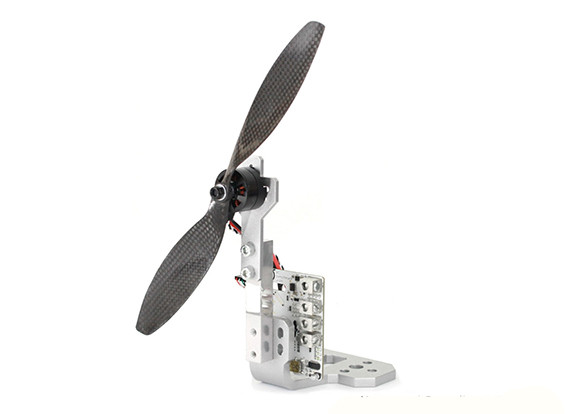
\includegraphics[width=0.5\textwidth]{Images/Propposed Aproach/TestBench.jpeg}
    \caption{Test bench used to measure the thrust and torque of the propeller.}
    \label{fig:Proposed Approach:Simulator:Testbench}
\end{figure}

To realize a fully holonomic robot with only six motors and propellers, it was necessary to utilize a combo of motors and ESC (electronic speed controller) capable of bidirectional operation. For the Space Cobot, this means that a CCW (counter-clockwise) propeller must also operate in the CW (clockwise) direction. While it is known that performance typically degrades when operating in the \enquote{wrong} direction, we simplified our model by post-processing the data to eliminate this loss of performance. The resulting thrust and torque curves are shown in Figure~\ref{fig:Proposed Approach:Simulation:MotorData}.

\begin{figure}[H]
    \begin{subfigure}{0.5\textwidth}
        \centering
        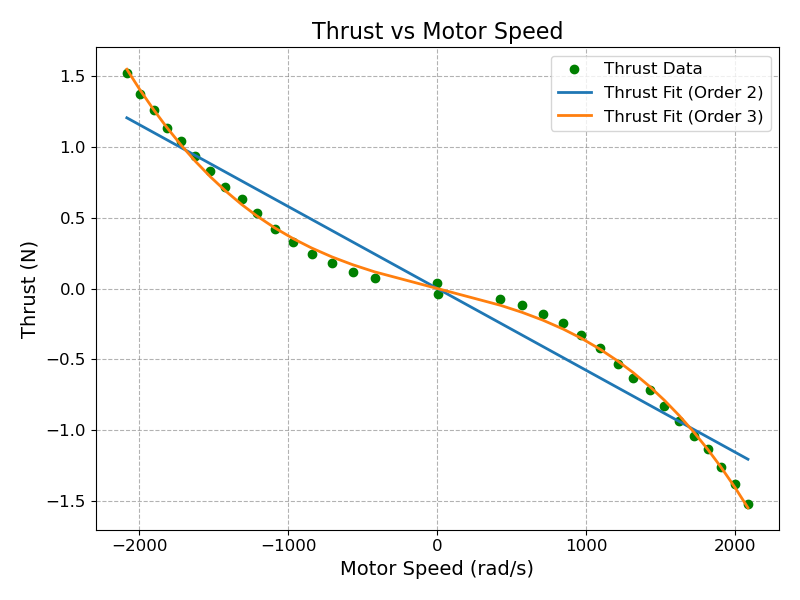
\includegraphics[width=0.9\textwidth]{Images/Propposed Aproach/thrust_vs_motor_speed.png}
        \caption{Thrust vs. motor speed.}
        \label{fig:proposed_approach_simulation_motor_data_thrust}
    \end{subfigure}
    \hfill
    \begin{subfigure}{0.5\textwidth}
        \centering
        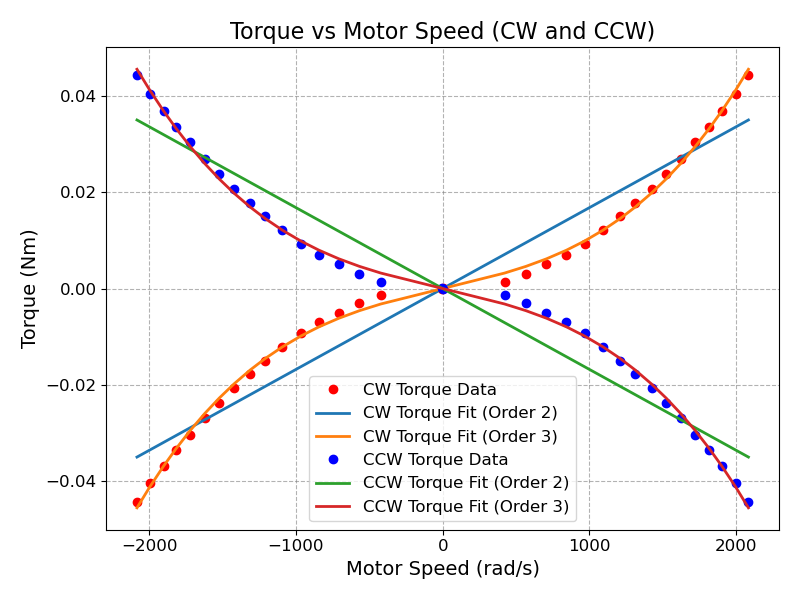
\includegraphics[width=0.9\textwidth]{Images/Propposed Aproach/torque_vs_motor_speed_CW_CCW.png}
        \caption{Torque vs. motor speed (CW and CCW).}
        \label{fig:proposed_approach_simulation_motor_data_torque}
    \end{subfigure}
    \caption{Thrust and torque data as functions of motor speed.}
    \label{fig:Proposed Approach:Simulation:MotorData}
\end{figure}

Upon analyzing the relationships between thrust and motor speed, as well as torque and motor speed, it became evident that a third-order polynomial provides the best fit. This conclusion is supported by the error metrics shown in Figure~\ref{fig:Proposed Approach:Simulation:FittingErrors}. The third-order fit achieves a substantial reduction in error compared to simpler models. Furthermore, higher-order models, such as the fourth-order fit, do not yield noticeable improvements. Specifically, the fourth-order fit effectively reduces to a third-order fit, with the fourth-order coefficient equating to zero, thus adding unnecessary complexity.

\begin{figure}[H]
    \begin{subfigure}{0.5\textwidth} 
        \centering
        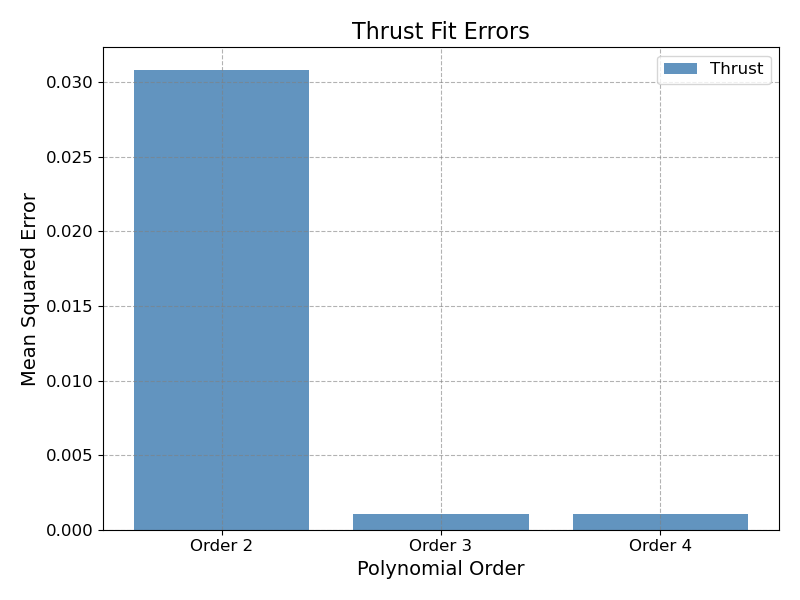
\includegraphics[width=0.9\textwidth]{Images/Propposed Aproach/thrust_errors.png}
        \caption{Thrust MSE between real data and fitted data.}
        \label{fig:Proposed Approach:Simulation:ThrustErrors}
    \end{subfigure} 
    \hfill
    \begin{subfigure}{0.5\textwidth}
        \centering
        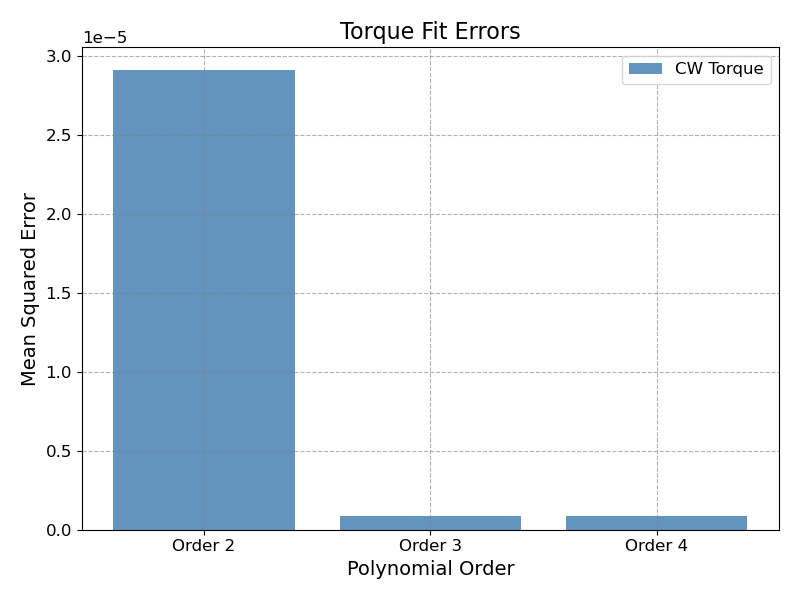
\includegraphics[width=0.9\textwidth]{Images/Propposed Aproach/torque_errors.png}
        \caption{Torque MSE between real data and fitted data.}
        \label{fig:Proposed Approach:Simulation:TorqueErrors}
    \end{subfigure}
    \caption{Mean Squared Error (MSE) between the real data and the fitted curves.}
    \label{fig:Proposed Approach:Simulation:FittingErrors}
\end{figure}
